\documentclass{article}[a4paper]
\usepackage[a4paper, total={6.5in, 9in}]{geometry}
\usepackage{float}
\usepackage{amsmath}
\usepackage{amssymb}
\usepackage{enumitem}
\usepackage{tabularray}
\usepackage{charter}
\usepackage{xcolor}
\usepackage{graphicx}
\usepackage{listings}
\usepackage{tikz}
\usepackage{parskip}
\usepackage[hidelinks]{hyperref}

\newcommand{\extlink}{
	
\begin{tikzpicture}[scale=0.1]
		\draw[rounded corners=0.5mm, line width=0.9pt] (-1, -1) rectangle (1, 1);
		\fill[white] (0, 0) rectangle (1.3, 1.3);
		\draw[line width=0.9pt, line cap=round] (0.15, 0.15) -- (1.3, 1.3);
		\draw[line width=0.9pt, line cap=round] (0.5, 1.3) -- (1.3, 1.3) -- (1.3, 0.5);
	\end{tikzpicture}
}

\lstset{
	language=Matlab,
	basicstyle=\ttfamily,
	keywordstyle=\color{blue},
	commentstyle=\color{gray},
	stringstyle=\color{red},
	showstringspaces=false,
	columns=fullflexible,
	breaklines=true,
	captionpos=b,
	backgroundcolor=\color[rgb]{0.96,0.96,0.96},
	xleftmargin=6pt,
	frame=tlbr,
	framesep=6pt,
	framerule=0pt,
}

\title{
	\huge{\textbf{
		Assignment 01
	}}\\
	\large{\phantom{}}\\
	\large{
		submitted for
	}\\
	\Large{
		\textbf{EN3551 - Digital Signal Processing}
	}\\
	\large{
		Department of Electronic and Telecommunication Engineering
	}
	\\
	\large{University of Moratuwa}
}

\author{
	\textbf{Udugamasooriya P. H. J.}\\
	220658U\\
	\small{Progress on \href{https://github.com/pulasthi-u/en3150-assignment01}{GitHub \extlink}}
}

\date{12 September 2025}

\begin{document}
	\maketitle
	
	\section{Harmonic Detection}
	
	\textbf{Question 03} Five subsets of the provided signal were formed as described. The magnitude plots of the DFTs of each of these subsets are indicated in Figure \ref{subset_dfts}.
	
	\begin{figure}[H]
		\centering
		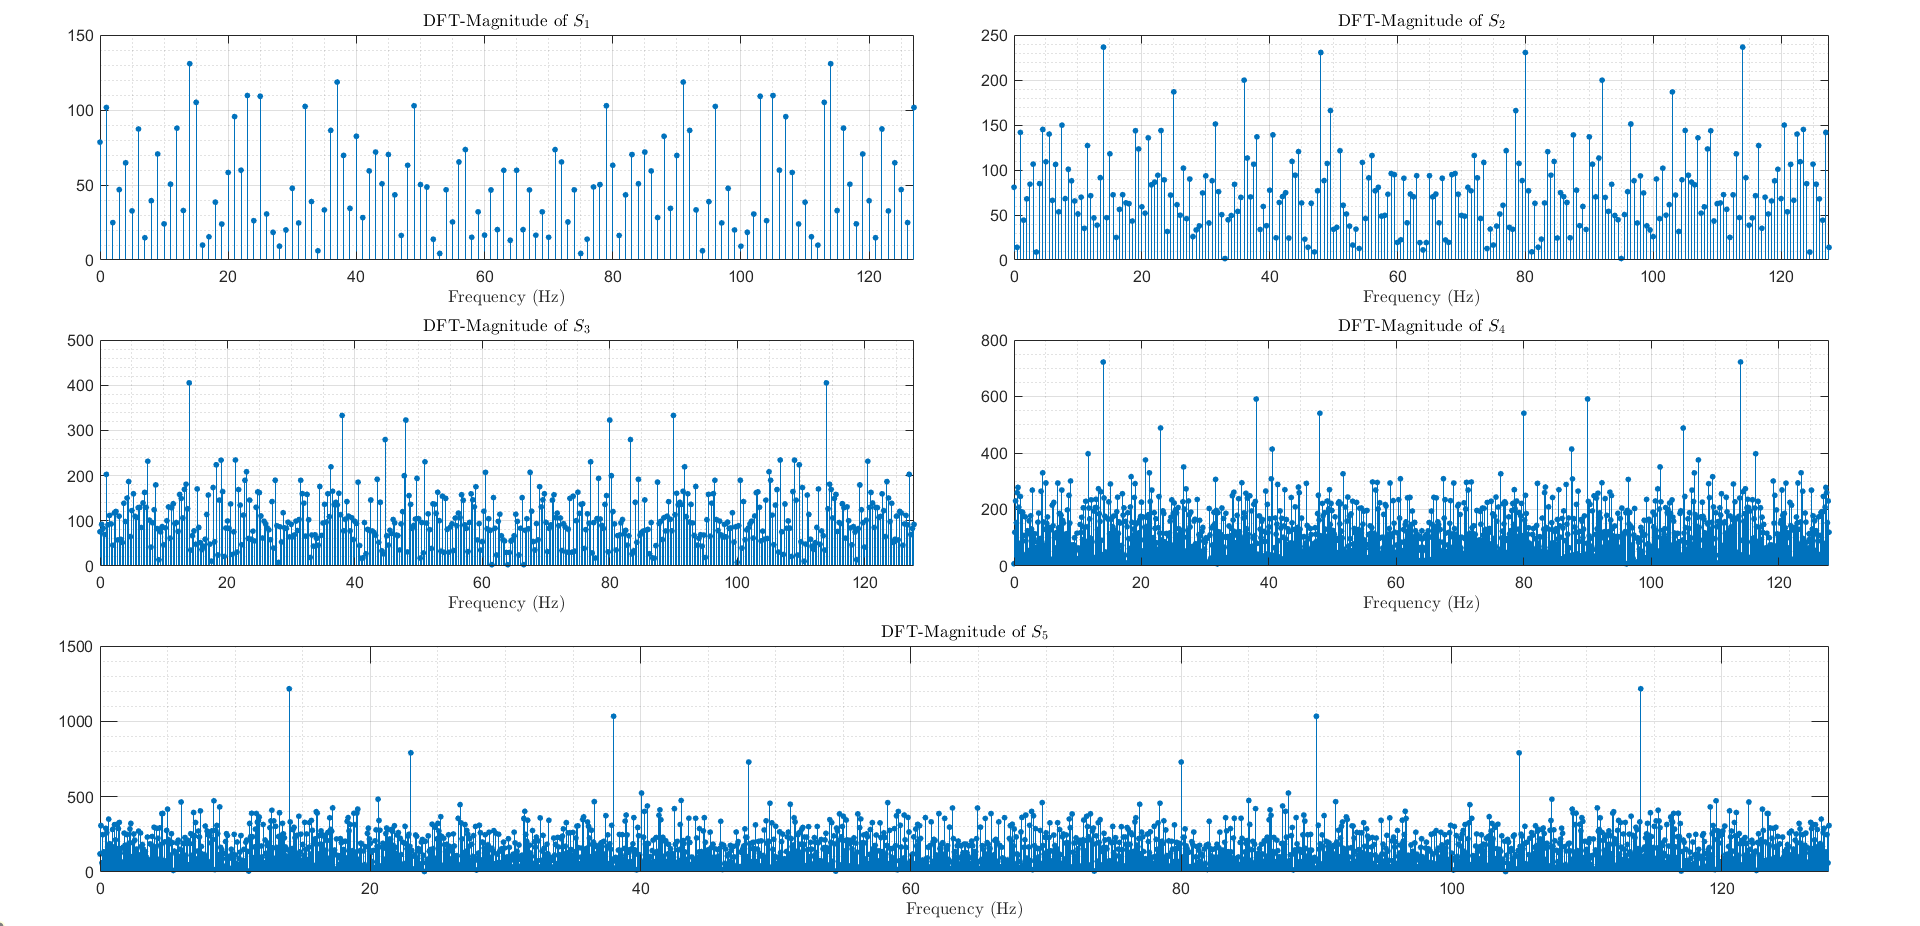
\includegraphics[width=\linewidth]{images/q1_3_1.png}
		\caption{DFT-magnitude plots of signals $S_1$ through $S_5$}
		\label{subset_dfts}
	\end{figure}
	
	To understand the differences between the DFTs above, we start by noting that an $N$-point signal $x[n]$ in the time domain will have an $N$-point DFT $X[k]$ in the frequency domain, related together through the inverse DFT relation as follows; \[
		x[n] = \dfrac{1}{N} \sum_{k=0}^{N-1} X[n] \cdot e^{j\frac{2\pi k}{N}n}, \text{ for } n = 0, \dots, N-1.
	\] We interpret the above expression as a decomposition of $x[n]$ into a linear combination of $N$ complex exponentials \[
		e^{j \omega_k n} = e^{j\frac{2\pi k}{N}n} \; (k = 1, \dots, N-1),
	\] where \[
		\omega_k = \frac{2\pi k}{N}.
	\] Notice that with bigger $N$, the frequencies of the complex exponentials that $x[n]$ is decomposed into become more closely and finely spaced. This means that a higher-order DFT can detect frequency content that simply goes undetected with a lower-order DFT.
	
	spectral leakage? other facts?
	
	specifically address the plots and say they show those effects
	
	For the problem of what harmonics are actually present, we look for the four most prominent spikes in the DFT of $S_5$; the signal whose DFT has the most clearly distinguishable spikes. These spikes are indicated in Figure \ref{dft_spikes}.
	
	\begin{figure}[H]
		\centering
		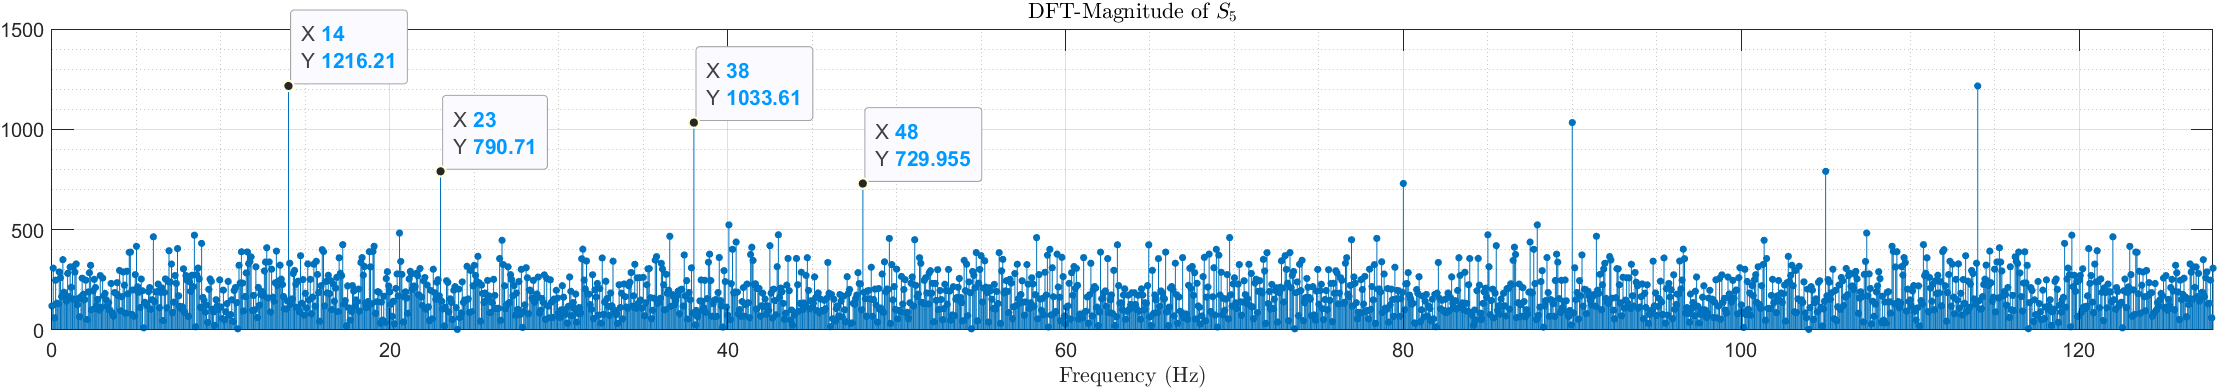
\includegraphics[width=\linewidth]{images/q1_3_1_peaks.png}
		\caption{Spikes in the DFT-magnitude plot of $S_5$}
		\label{dft_spikes}
	\end{figure}
	
	We conclude therefore that the harmonics present are $\mathbf{14}\textbf{ Hz}$, $\mathbf{23}\textbf{ Hz}$, $\mathbf{38}\textbf{ Hz}$ and $\mathbf{48}\textbf{ Hz}$.
	\medskip
	
	\textbf{Question 04} We use this code. Figure \ref{avg_dft} shows the magnitude plot resulting from averaging the DFTs of $L = 14$ consecutive subsets taken from the given signal, with the most prominent spikes selected.
	
	\begin{figure}[H]
		\centering
		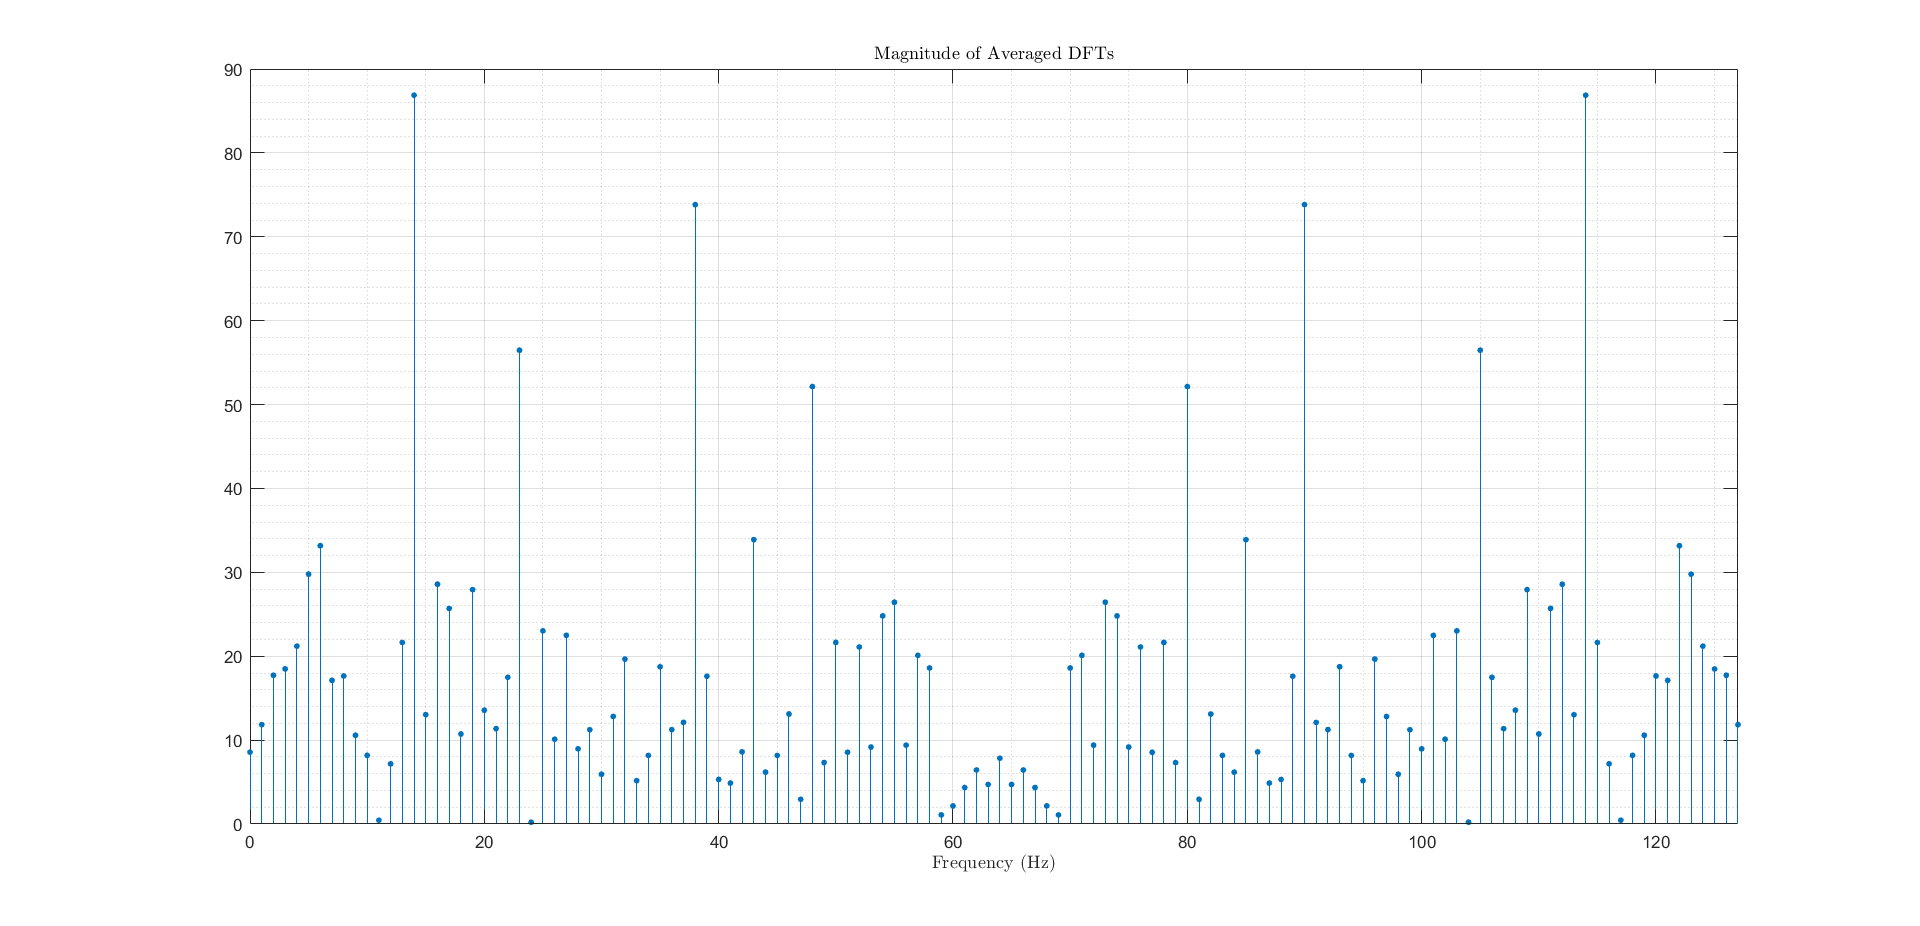
\includegraphics[width=\linewidth]{images/q1_3_2.png}
		\caption{Magnitude plot of the averaged DFT over several subsets}
		\label{avg_dft}
	\end{figure}
	
	We observe that the above plot is a much clearer plot, with the same frequencies $\mathbf{14}\textbf{ Hz}$, $\mathbf{23}\textbf{ Hz}$, $\mathbf{38}\textbf{ Hz}$ and $\mathbf{48}\textbf{ Hz}$ as detected before standing out prominently.
	
	To analyze this procedure, let us start by denoting the clean signal by $s[n]$ and the Gaussian noise (assumed AWGN) by $w[n]$, so that the observed signal, which we will denote $x[n]$ is given by \[
		x[n] = s[n] + w[n], \text{ for } n = 1, \dots, N-1,
	\] where in our case, $N = 1792$. Note that $w[n]$ is a random variable for each $n$; we assume that all the $w[n]$'s are independent, normally distributed (iid) random variables, with zero mean and some variance $\sigma^2$. It follows then that $x[n]$ is also a random variable for each $n$.
	
	Denote by $X\left(e^{j\omega}\right)$ the following: \[
		X\left(e^{j\omega}\right)
		=
		\sum_{n=0}^{N-1} x[n] \cdot e^{-j\omega n},
	\] and let $S\left(e^{j\omega}\right)$ and $W\left(e^{j\omega}\right)$ be defined similarly. Note that $S\left(e^{j\omega}\right)$ is precisely the DTFT of $s[n]$, whereas $X\left(e^{j\omega}\right)$ and $W\left(e^{j\omega}\right)$ are linear combinations of iid Gaussian random variables.
	
	Now, observe that \[
		X\left(e^{j\omega}\right)
		=
		\sum_{n=0}^{N-1} x[n] \cdot e^{-j\omega n}
		=
		\sum_{n=0}^{K-1} x[n] \cdot e^{-j\omega n}
		+
		\sum_{n=K}^{2K-1} x[n] \cdot e^{-j\omega n}
		+
		\cdots
		+
		\sum_{n=\frac{N}{K} - 1}^{N-1} x[n] \cdot e^{-j\omega n},
	\] where we break the sum defining $X\left(e^{j\omega}\right)$ into smaller sums taken over smaller subsets of $x[n]$, each having $K$ samples. Let us denote a general term in the above sum by \[
		X_a\left(e^{j\omega}\right)
		=
		\sum_{n=aK}^{(a+1)K-1} x[n] \cdot e^{-j\omega n},
	\] so that \[
		X\left(e^{j\omega}\right)
		=
		\sum_{a=0}^{\frac{N}{K}-1} X_a\left(e^{j\omega}\right).
	\]
	
	Note that
	\begin{align*}
		X_a\left(e^{j\omega}\right)
		&=	\sum_{n=aK}^{(a+1)K-1} x[n] \cdot e^{-j\omega n} \\
		&=	\sum_{n=0}^{K-1} x[n + aK] \cdot e^{-j\omega (n + aK)} \\
		&=	e^{-j\omega aK} \sum_{n=0}^{K-1} x[n + aK] \cdot e^{-j\omega n}.
	\end{align*}
	By letting \[
		X_{aK} \left(e^{j\omega}\right) = \sum_{n=0}^{K-1} x[n + aK] \cdot e^{-j\omega n},
	\] and putting all this together, using linearity properties, we find that
	\begin{align*}
		S\left(e^{j\omega}\right)
		&=	X\left(e^{j\omega}\right) - W\left(e^{j\omega}\right) \\
		\sum_{a=0}^{\frac{N}{K}-1} S_a\left(e^{j\omega}\right)
		&=	\sum_{a=0}^{\frac{N}{K}-1} X_a\left(e^{j\omega}\right)
			-
			\sum_{a=0}^{\frac{N}{K}-1} W_a\left(e^{j\omega}\right) \\
		\sum_{a=0}^{\frac{N}{K}-1} e^{-j\omega aK} \cdot S_{aK} \left(e^{j\omega}\right)
		&=	\sum_{a=0}^{\frac{N}{K}-1} e^{-j\omega aK} \cdot X_{aK} \left(e^{j\omega}\right)
			-
			\sum_{a=0}^{\frac{N}{K}-1} e^{-j\omega aK} \cdot W_{aK} \left(e^{j\omega}\right).
	\end{align*}
	
	Setting $\omega = \dfrac{2\pi k}{K}$ ($k = 1, \dots, K-1$), we obtain \[
		S\left(e^{j\frac{2\pi k}{K}}\right)
		=
		\sum_{a=0}^{\frac{N}{K}-1} \cdot S_{aK} \left(e^{j\omega}\right)
		=
		\sum_{a=0}^{\frac{N}{K}-1} X_{aK} \left(e^{j\frac{2\pi k}{K}}\right)
		-
		\sum_{a=0}^{\frac{N}{K}-1} W_{aK} \left(e^{j\frac{2\pi k}{K}}\right),
	\] because $e^{-j\frac{2\pi k}{K} aK} = e^{-j 2\pi ak} = 1$, for any integer $a$ and $k$.
	
	Define $X[k]$ for $k=1,\dots,N-1$ by \[
		X_{aK}[k] = \sum_{n=0}^{K-1} x[n + aK] \cdot e^{-j\frac{2\pi}{K} kn},
	\] and let $S[k]$ and $W[k]$ also be defined similarly. Noting that $X_{aK}[k] = X_{aK} \left(e^{j\frac{2\pi}{K} k}\right)$, we can then also write \[
		S\left(e^{j\frac{2\pi k}{K}}\right)
		=
		\sum_{a=0}^{\frac{N}{K}-1} \cdot S_{aK} [k]
		=
		\sum_{a=0}^{\frac{N}{K}-1} X_{aK} [k]
		-
		\sum_{a=0}^{\frac{N}{K}-1} W_{aK} [k].
	\] Finally, dividing through by $\dfrac{N}{K}$ yields \[
		\dfrac{K}{N} S\left(e^{j\frac{2\pi k}{K}}\right)
		=
		\dfrac{K}{N} \sum_{a=0}^{\frac{N}{K}-1} \cdot S_{aK} [k]
		=
		\dfrac{K}{N} \sum_{a=0}^{\frac{N}{K}-1} X_{aK} [k]
		-
		\dfrac{K}{N} \sum_{a=0}^{\frac{N}{K}-1} W_{aK} [k].
	\]
	
	But, note that \[
		W_{aK}[k] = \sum_{n=0}^{K-1} w[n + aK] \cdot e^{-j\frac{2\pi k}{K} n},
	\] where the $w[n + aK]$'s are iid Gaussian random variables. Hence, it follows that $W_{aK}[k]$ is itself a Gaussian random variable. It is easy to see that due to the iid assumption, the $W_{aK}[k]$'s are also iid, for each $a$ and $k$.
	
	We note specifically that each $W_{aK}[k]$ is Gaussian with mean \[
		\mathbb{E}\left(W_{aK}[k]\right)
		=
		\sum_{n=0}^{K-1} \mathbb{E}\left(w[n + aK]\right) \cdot e^{-j\frac{2\pi k}{K} n}
		= 0,
	\] and we know that the sample mean over any finite set of observed $W_{aK}[k]$'s is an unbiased estimator of this mean, whose value approaches the true mean as the number of observations increases.
	
	The term \[
		\dfrac{K}{N} \sum_{a=0}^{\frac{N}{K}-1} W_{aK} [k]
	\] in the expression derived above is exactly the sample mean of some observed values of $W_{aK}[k]$'s once the signal $x[k]$ is given, and \[
		\dfrac{K}{N} \sum_{a=0}^{\frac{N}{K}-1} X_{aK} [k]
	\] is the average of $\dfrac{N}{K}$ $K$-point DFTs taken over $\dfrac{N}{K}$ consecutive subsets of $x[n]$.
	
	Hence, we have shown that the averaging process lets us approximate $S\left(e^{j\frac{2\pi k}{K}}\right)$ from an AWGN-corrupted signal by acting to reduce the impact of AWGN.
	\medskip
	
	\textbf{Question 05} Reducing $L$ while holding $K$ constant has the effect of dropping out samples from the signal.
	\medskip
	
	\textbf{Question 06} can any value of K be used?
	
	\section{Interpolation}
	
	\textbf{Question 01} A plot of the first 50 samples of the loaded original signal is given in Figure \ref{orig_x1}.
	
	\begin{figure}[H]
		\centering
		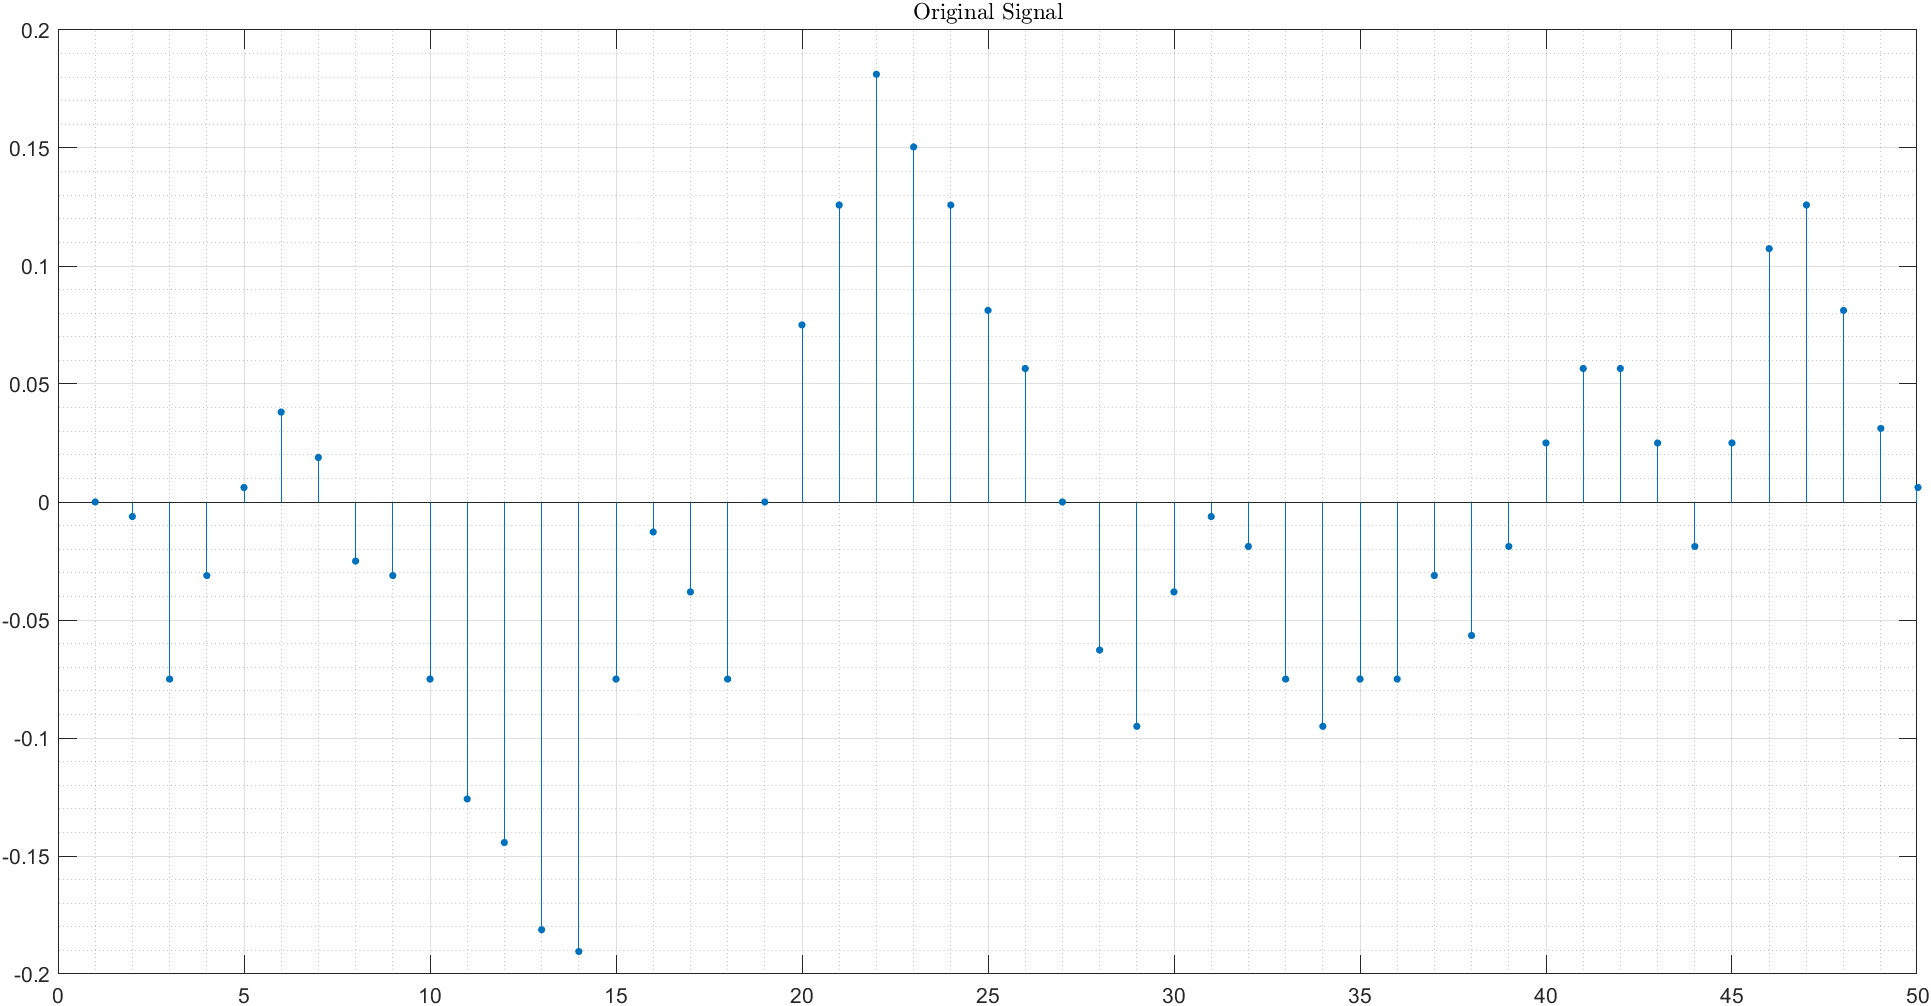
\includegraphics[width=0.9\linewidth]{images/q2_orig_sig.png}
		\caption{Original signal}
		\label{orig_x1}
	\end{figure}
	
	\textbf{Question 03} Steps (a) through (c) were carried out using the code in Listing X in Appendix \ref{code}. Outputs obtained from the code and relevant plots are as shown in Listings \ref{x2_x_norm}, \ref{x3_x_norm}, \ref{x4_x_norm} and Figures \ref{x2_interp}, \ref{x3_interp}, and \ref{x4_interp} respectively.
	
	In each figure, we plot the interpolated version of the signal first, and then superimpose it on the original signal to allow for better comparison.
	
	An analysis of the results obtained follows.
	
	\begin{enumerate}[label=(\alph*)]
		\item \phantom{a}
		\begin{figure}[H]
			\centering
			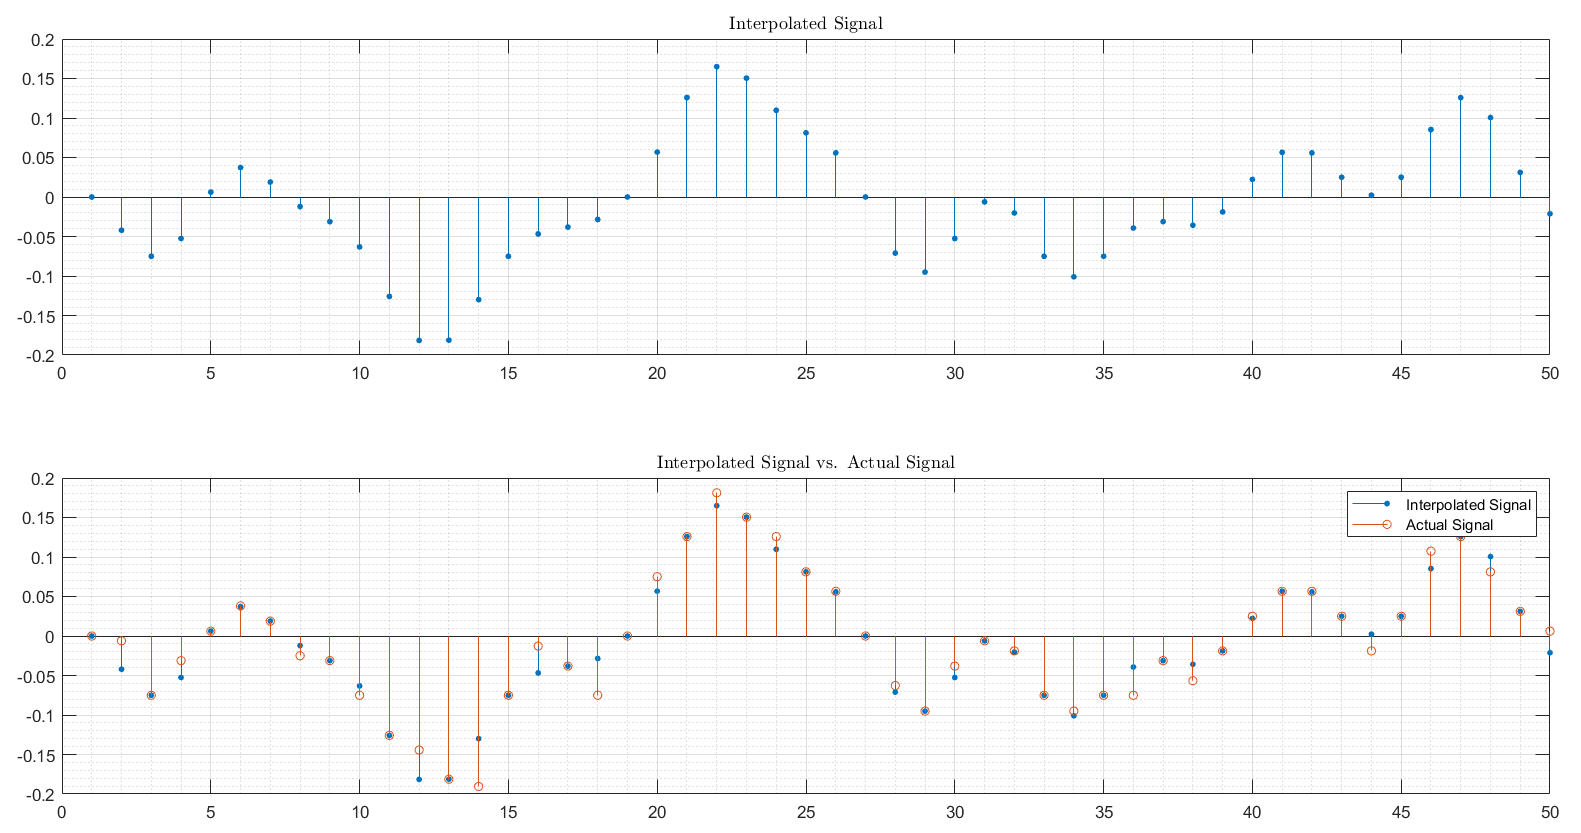
\includegraphics[width=0.9\textwidth]{images/q2_x2_interp.png}
			\caption{$x_2$ Interpolated}
			\label{x2_interp}
		\end{figure}
		
		\begin{lstlisting}[caption={Code output}, label=x2_x_norm]
Norm of difference: 6.1447
		\end{lstlisting}
		
		\item \phantom{a}
		\begin{figure}[H]
			\centering
			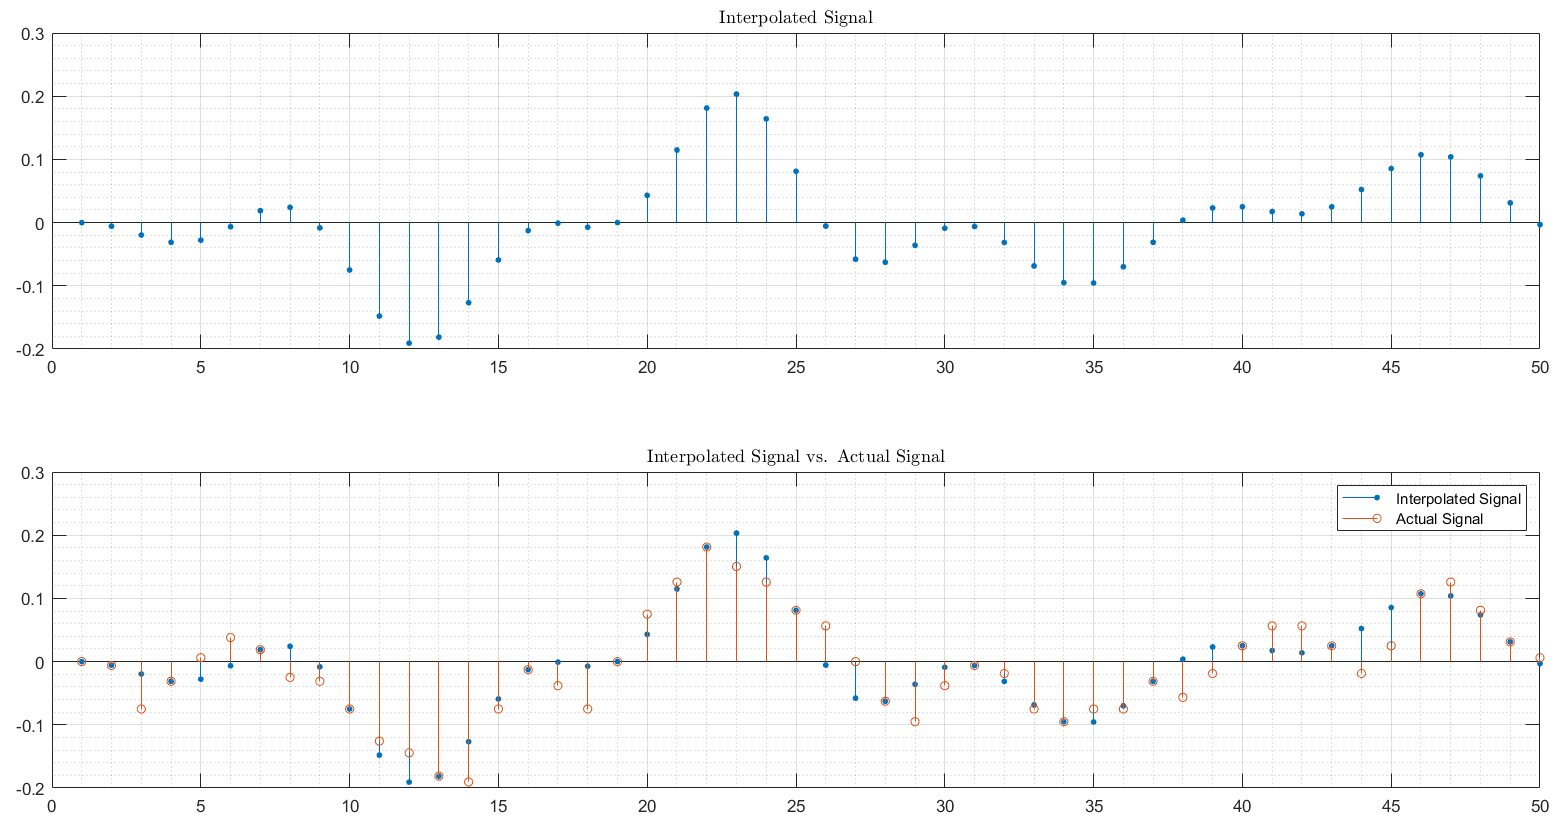
\includegraphics[width=0.9\textwidth]{images/q2_x3_interp.png}
			\caption{$x_3$ Interpolated}
			\label{x3_interp}
		\end{figure}
		
		\begin{lstlisting}[caption={Code output}, label=x3_x_norm]
Norm of difference: 8.3652
		\end{lstlisting}
		
		\item \phantom{a}
		\begin{figure}[H]
			\centering
			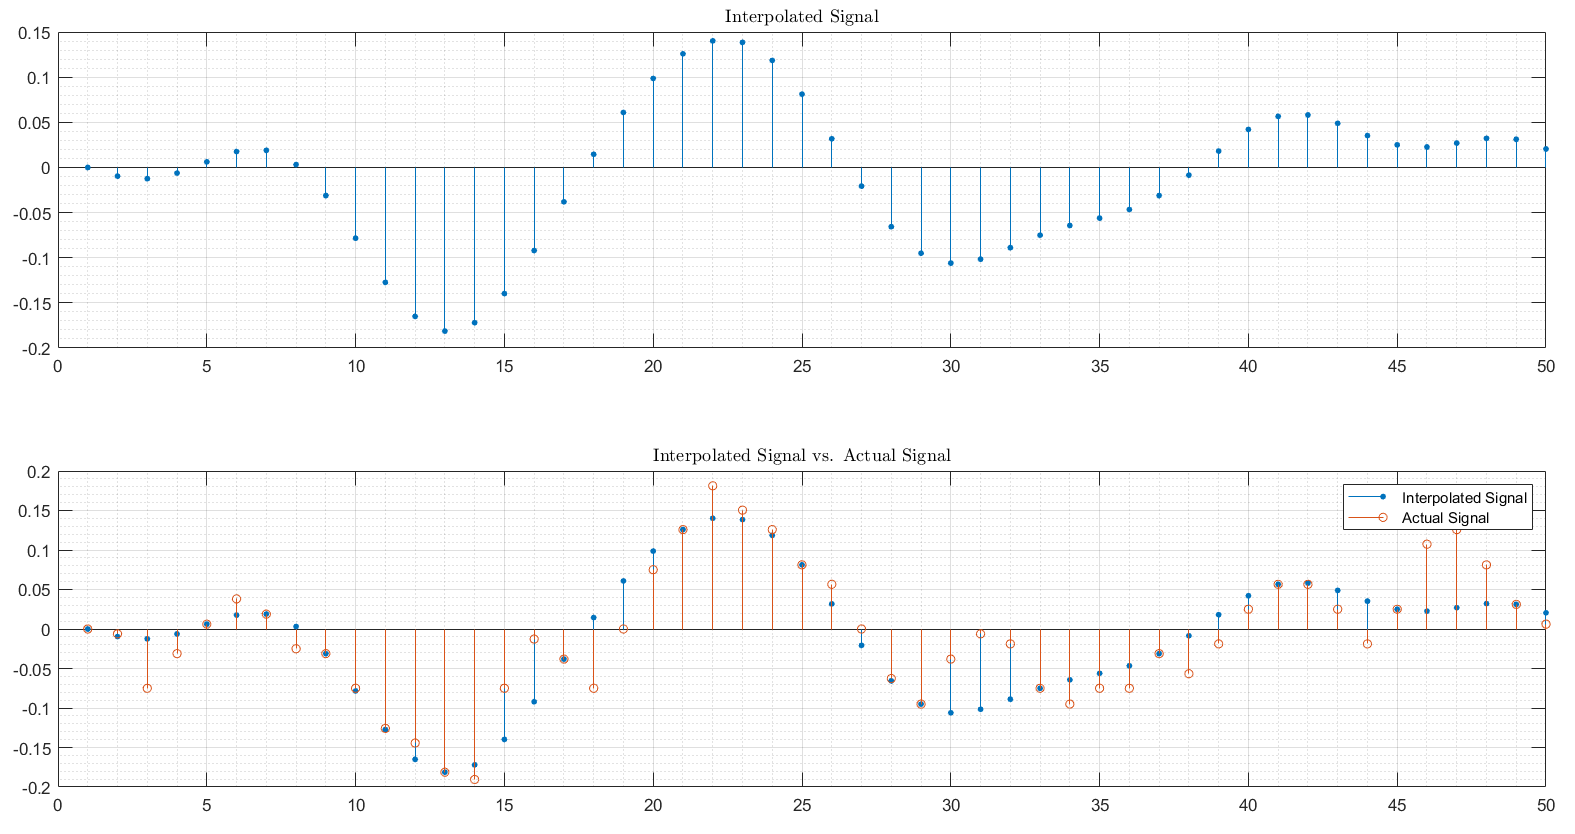
\includegraphics[width=0.9\textwidth]{images/q2_x4_interp.png}
			\caption{$x_4$ Interpolated}
			\label{x4_interp}
		\end{figure}
		
		\begin{lstlisting}[caption={Code output}, label=x4_x_norm]
Norm of difference: 23.4998
		\end{lstlisting}
		
		\item Figure \ref{all_compare} shows a plot of the original signal, each interpolated signal separately, and finally, a superimposition of all of the above.
		
		\begin{figure}[H]
			\centering
			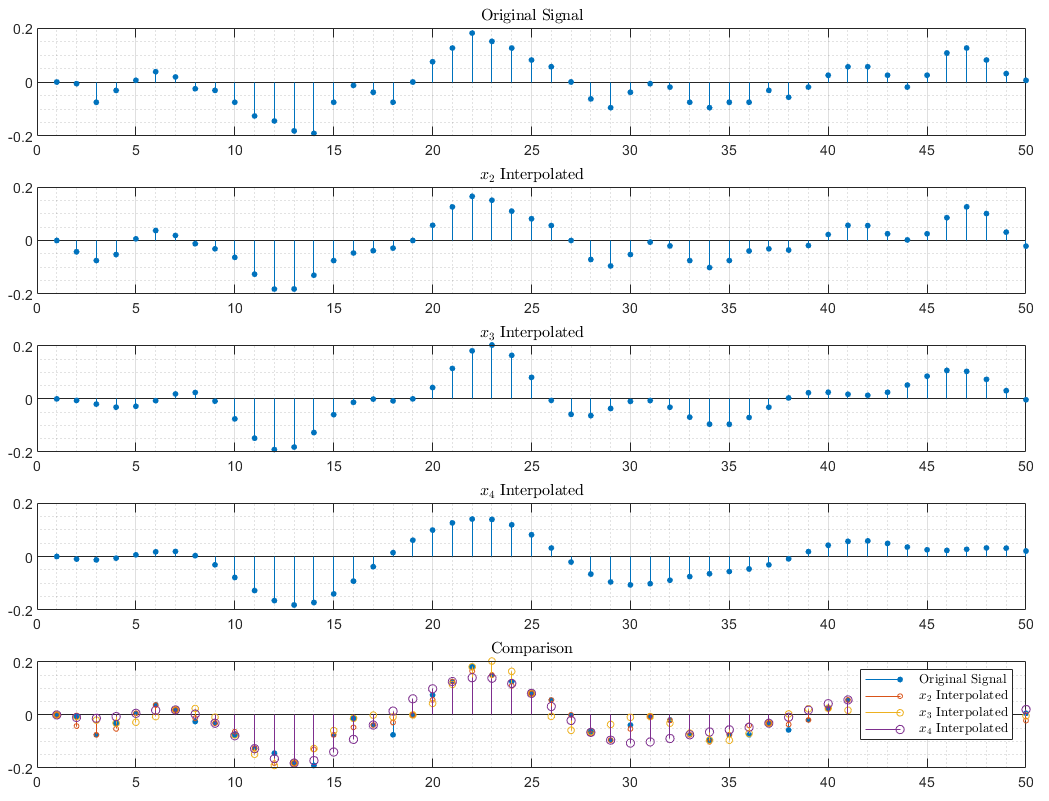
\includegraphics[width=\linewidth]{images/q2_all_compare.png}
			\caption{Comparison of original signal against all interpolated versions}
			\label{all_compare}
		\end{figure}
		
		
	\end{enumerate}
	
	\appendix
	\section{Code Snippets}
	\label{code}
	
	\subsection{Harmonic Detection}
	
	\subsection{Interpolation}
	
\end{document}